
%% Blessings

\newcommand{\startblessingstable}{\par\begin{minipage}{\textwidth}\raggedcolumns\begingroup\setlength{\columnsep}{5pt}\begin{multicols}{3}}

\newcommand{\newblessing}[3]{%
	\begin{center}%
		\includegraphics[width=0.72\columnwidth]{pics/#1sblessing.png}\vspace*{2pt}\par%
		\textbf{#2}%
		\def\tempENname{}%
		\StrGobbleRight{\expandafter\expandafter\expandafter\@gobble\expandafter\string#2}{1}[\tempENname]%
		\expandafter\ifundef\expandafter{\csname \tempENname EN\endcsname}{% then there is nothing to add
		}{%
			\newline\textit{(\csname \tempENname EN\endcsname)}%
		}
		\vspace*{3pt}\par%
		#3%
	\end{center}\columnbreak%
}

\newcommand{\closeblessingtable}{\end{multicols}\endgroup\end{minipage}\vspace*{-12pt}}

%% Orders

\newcommand{\startorderstable}{%
\renewcommand{\arraystretch}{1.4}%
\DTLifdbexists{orderslist}{\DTLcleardb{orderslist}}{\DTLnewdb{orderslist}}% Create new/discard old list
\vspace*{3pt}\par%
\begin{minipage}[c]{0.75\textwidth}\begin{center}\begin{tabular}{>{\raggedleft}m{3.3cm}m{8.6cm}}%
\toprule
}

\newcommand{\closeorderstable}{%
\DTLsort*{sortlabel}{orderslist}% Sort list
\DTLforeach*{orderslist}{\name=name,\ruletext=ruletext}{%
\textbf{\name}&\ruletext{}\DTLiflastrow{}{\tabularnewline}%
}
\tabularnewline\bottomrule
\end{tabular}\end{center}\end{minipage}%
\hfill\begin{minipage}[c]{0.22\textwidth}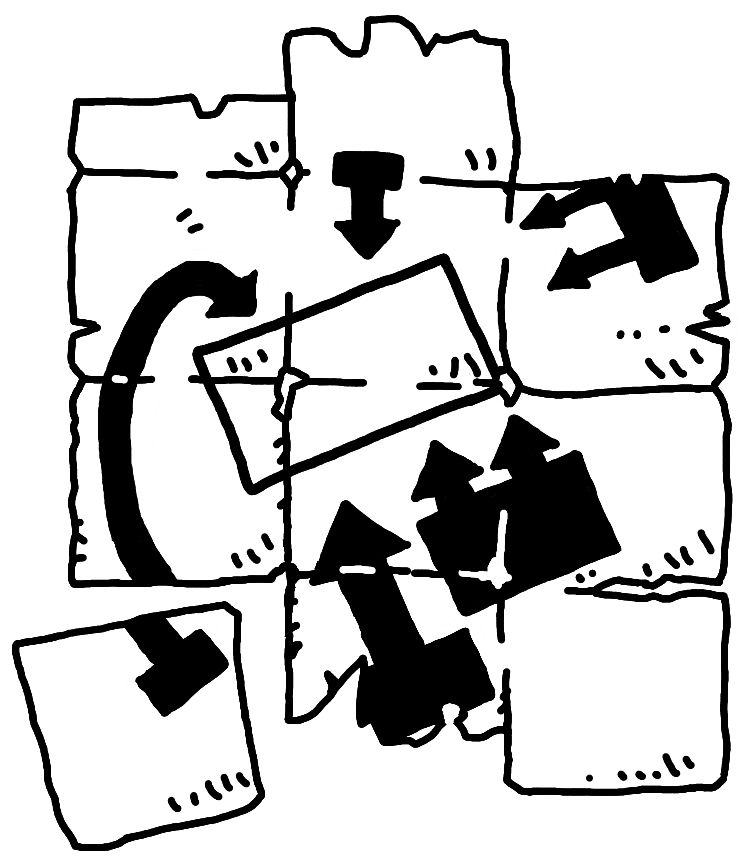
\includegraphics[width=\textwidth]{pics/orders.jpg}\end{minipage}%
\DTLcleardb{orderslist}\debugfooter%
}

\newcommand{\addorder}[2]{%
	\DTLnewrow{orderslist}%
	\pdfstringdef\textwithoutformatting{#1}%
	\pdfsubstitute\textwithoutformatting{'}{}%
	\pdfsubstitute\textwithoutformatting{ }{}%
	\dolanguagespecificsubstitute{}%
	\def\DTLentrycommand{\DTLnewdbentry{orderslist}{sortlabel}}%
	\expandafter\DTLentrycommand\expandafter{\textwithoutformatting}%
	\DTLnewdbentry{orderslist}{name}{#1}%
	\DTLnewdbentry{orderslist}{ruletext}{#2}%
}
